\begin{frame}{File Storage - What is it }

\begin{columns}
    \begin{column}{0.47\textwidth}
    \begin{block}{File Storage}
        \begin{itemize}
            \item Hierarchical Structure 
            \item Files, Folders, Sub-directories, Directories
            \item Good with structured data 
            \item Filesystem
        \end{itemize}
    \end{block}
    \end{column}
    \begin{column}{0.47\textwidth}
        \begin{figure}
        \centering
        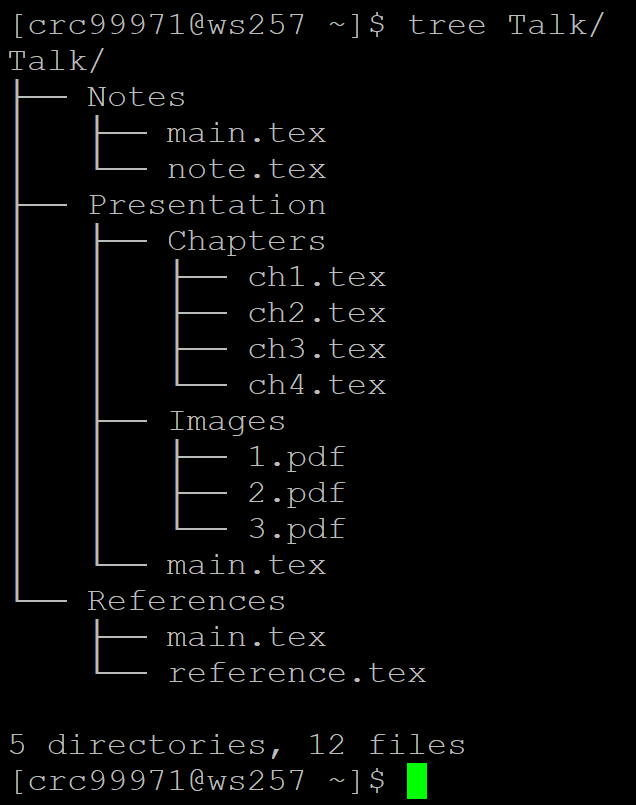
\includegraphics[width=\textwidth,height=0.7\textheight,keepaspectratio]{img/tree.PNG}
        \caption{File Storage}
        \label{fig:my_label}
    \end{figure}
    \end{column}
\end{columns}
\end{frame}
\note{So what about unstructured data, i.e images}

\begin{frame}{File Storage - Unstructured data}
    \begin{figure}
        \centering
        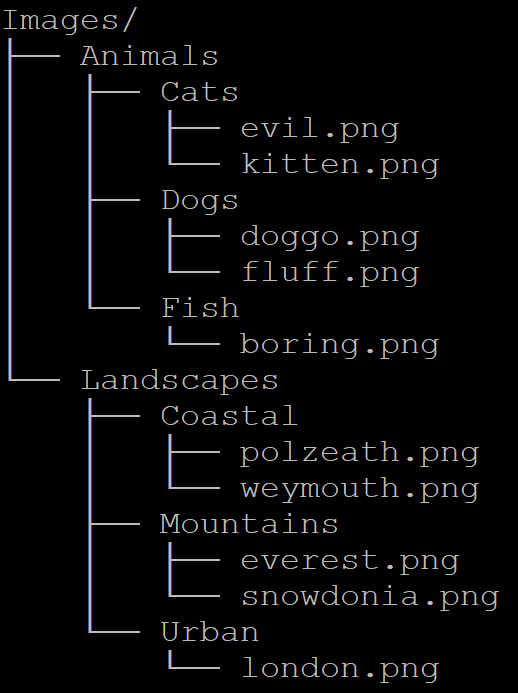
\includegraphics[width=\textwidth,height=0.7\textheight,keepaspectratio]{img/image-tree.png}
        \caption{Image Folder}
        \label{fig:my_label}
    \end{figure}  
\end{frame}


\begin{frame}{File Storage - Storing Images}
\begin{columns}
    \begin{column}{0.47\textwidth}
    \begin{figure}
        \centering
        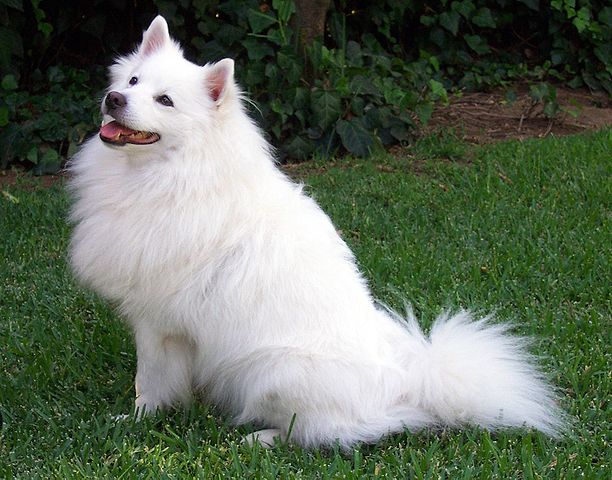
\includegraphics[width=\textwidth,height=0.45\textheight,keepaspectratio]{img/dog.jpg}
        \label{fig:my_label}
    \end{figure}
    \end{column}
    \begin{column}{0.47\textwidth}
    \begin{figure}
        \centering
        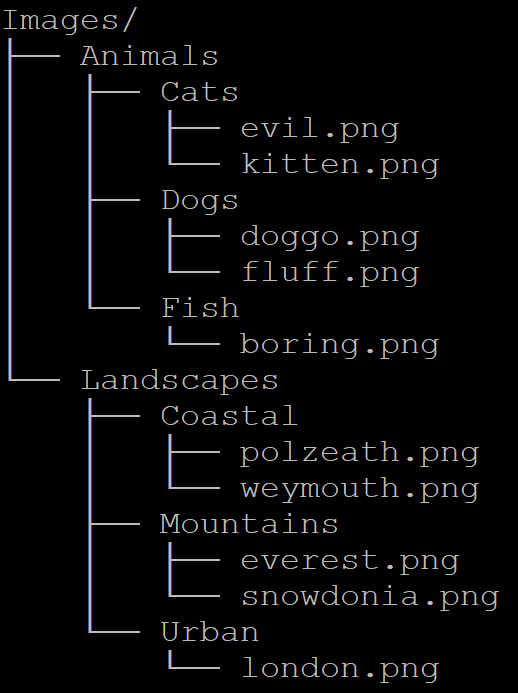
\includegraphics[width=\textwidth,height=0.55\textheight,keepaspectratio]{img/image-tree.png}
        \label{fig:my_label}
    \end{figure}
    \end{column}
\end{columns} 
\begin{block}{Where to store}
\begin{description}
    \item [A] Images/Animals/Dogs
    \item [B] Images/Animals/Cats
    \item [C] Images/Landscapes/Urban
\end{description}
\end{block}
\end{frame}
\note{If we have a file-system for storing images, that has subdirectories, Landscapes and Animals, and say Landscapes has subdirectories of Coastal, Mountain, Urban, etc. and Animals has subdirectories of; Fish, Dogs, Cats, etc. Now if we have well-defined images, of just Dogs, Coasts, Mountains and Cats. This system works perfectly well.}
\begin{frame}{File Storage - Storing Images}
\begin{columns}
    \begin{column}{0.47\textwidth}
    \begin{figure}
        \centering
        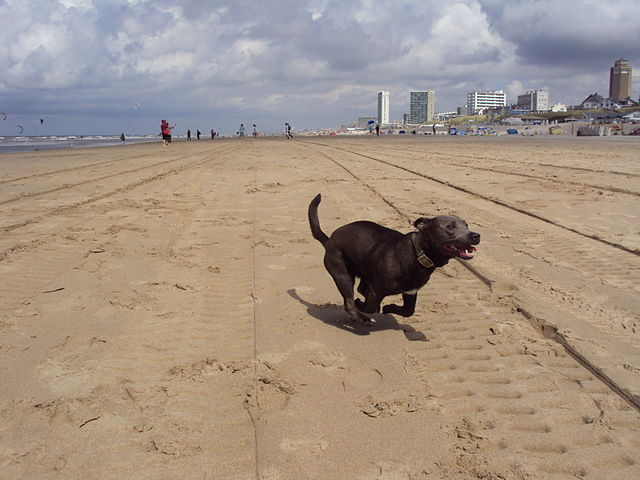
\includegraphics[width=\textwidth,height=0.45\textheight,keepaspectratio]{img/dog-or-beach.jpg}
        \label{fig:my_label}
    \end{figure}
    \end{column}
    \begin{column}{0.47\textwidth}
    \begin{figure}
        \centering
        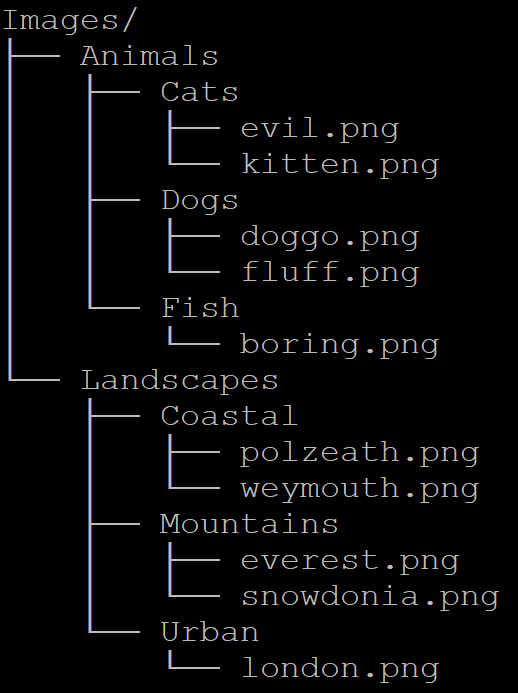
\includegraphics[width=\textwidth,height=0.55\textheight,keepaspectratio]{img/image-tree.png}
        \label{fig:my_label}
    \end{figure}
    \end{column}
\end{columns} 
\begin{block}{Where to store}
\begin{description}
    \item [A] Images/Animals/Dogs
    \item [B] Images/Landscapes/Coastal
    \item [C] Images/Landscapes/Urban
\end{description}
\end{block}
\end{frame}
\note{However, if we have an image of a Dog at the Beach, where do you place this image within this structure. It could either go in the Dogs or Coastal directory either would make sense. However, when looking for that image again, are you going to have remembered where you put it. Object Storage would make sense here as the data doesn't have an inherent structure as much as we can try.}


\begin{frame}{File Storage - Pros and Cons}
\begin{columns}[t]
    \begin{column}{0.47\textwidth}
    \begin{block}{Pros}
        \begin{itemize}
            \item Stores data in  Hierarchical structure
            \item Ideal for structured data
            \item Human interpretable 
            \item Already in use at Diamond (GPFS)
        \end{itemize}
    \end{block}
    \end{column}
    \begin{column}{0.47\textwidth}
    \begin{block}{Cons}
        \begin{itemize}
            \item Not good with unstructured data
            \item File Size issues
            \item Lots of files
            \item Not Cloud native
            \item Expensive
        \end{itemize}
    \end{block}
    \end{column}
\end{columns}
\end{frame}



\note{So there are pros to using a File Storage, it handles data that has implicit structure very well, it can scale, and we already have the infrastructure in place for it. There are cons being that it struggles with lots of small files, performance dip. However those are problems that make sense to deal with if you are dealing with structured data. However, Diamond does not really deal with structured data. We deal with images, which don't in heartily have a structure. 


}